\chapter{Introducing the interplay between questions and assertions}\label{chap:introduction}


Assertions and questions form the two core, dual components of natural language. Question typically request information, while assertions typically provide information. (\ref{ex:simple-q}) for instance, is a question that requests information about the country where Jo grew up (presupposing there is one such country). (\ref{ex:simple-a}) can be seen as a good (assertive) answer to this question, providing the piece of information that Jo grew up in France.

\begin{exe}
	\ex\label{ex:simple-q-a}
	\begin{xlist}
		\ex {In which country did Jo grow up?}\label{ex:simple-q}
		\ex {--Jo grew up in France.}\label{ex:simple-a}
	\end{xlist}
\end{exe}

\section{Assertions provide information in the form of propositions}

When studying the semantics of natural language expressions, one usually starts with assertions, because they appear intuitively simpler. We will use the simple assertion in (\ref{ex:simple-a}), as a running example. At the most basic level, assertions are truth-conditional, i.e. their meaning corresponds to the set of conditions under which they hold. For instance, \textit{Jo grew up in France} will be true if an only if whoever \textit{Jo} is, grew up in whatever geographical entity \textit{France} is. The \textit{extension} of an assertion is therefore of type \texttt{t}, the type of truth-conditions.

Additionally, the truth-conditions of a sentence are parametrized by (at least) a world variable.\footnote{Other parameters can also be relevant, like times, and assignments. But we choose to keep things simple here.}. So, \textit{Jo grew up in France} will be true as evaluated against a world $w_0$ if an only if whoever \textit{Jo} is in $w_0$, grew up in $w_0$ in whatever geographical entity \textit{France} is in $w_0$. One can then abstract over this world-parameter, and define the \textit{intension} of an assertion as a function from worlds to truth-conditions. Such functions are called \textit{propositions}, and have type $\langle \texttt{s}, \texttt{t}\rangle$, where \texttt{s} is the type of world-variables. So, the intension, or propositional content of \textit{Jo grew up in France}, will be a function mapping any world variable $w$, to the truth condition yielding true if an only if, whoever \textit{Jo} is in $w$, grew up in $w$ in whatever geographical entity \textit{France} is in $w$. This is formalized (with some simplifications) in (\ref{ex:prop-func}).

\begin{exe}
	\ex {$\llbracket$ Jo grew up in France $\rrbracket$ = $\lambda w. \ $ Jo grew up in France in $w$\\
		\phantom{$\llbracket$ Jo grew up in France $\rrbracket$} : $\langle \texttt{s}, \texttt{t}\rangle$}\label{ex:prop-func}
\end{exe}

Propositions can receive an alternative, equivalent interpretation in terms of sets, based on the idea that any function with domain $D$ and range $R$ is just a (potentially infinite) set of pairs of elements in $D\times R$. A proposition is then simply the set of worlds in which it holds. This interpretation of propositions will be heavily used throughout the dissertation, and is outlined in (\ref{ex:prop-func-set}). 

\begin{exe}
	\ex {$\llbracket$ Jo grew up in France $\rrbracket$ = $\lambda w. \ $ Jo grew up in France in $w$\\
		\phantom{$\llbracket$ Jo grew up in France $\rrbracket$} $\simeq$ $\lbrace w \ | \ $ Jo grew up in France in $w$ $\rbrace$}\label{ex:prop-func-set}
\end{exe}

Proposition either denote functions of type $\langle \texttt{s}, \texttt{t}\rangle$, or subsets of the set of elements of type \texttt{s}. Should all elements of type \texttt{s} be considered when evaluating such functions, or computing such subsets? It is commonly assumed that the worlds under consideration at any point of a conversation, are the ones that are compatible with the premises of the said conversation. For instance, if two people have a discussion about \textit{France}, it is often reasonable to assume that they agree on what geographical area \textit{France} encompasses, and more generally about the topology of Earth. Moreover, they agree that they agree on this; and agree that they agree that they agree on this; etc. Propositions subject to this recursive, mutual, tacit agreement pattern, form what is called a Common Ground (henceforth \textbf{CG}, \citep{Stalnaker1974, Stalnaker1978}). Each conversation has its own CG, as defined in (\ref{ex:common-ground}). The set of worlds in which all the propositions of the CG hold, is called the Context Set (henceforth \textbf{CS}). The CS associated with a conversation is therefore a subset of the set of all possible worlds; and can also be seen (under the set interpretation of propositions) as the grand intersection of the propositions in the CG. This is defined in (\ref{ex:context-set}). We will often refer to this set as \textit{the} CS, taken for granted a generic conversation and CG.

\begin{exe}
	\ex {\textit{Common Ground (\textbf{CG}).} Let $\mathcal{C}$ be a conversation between participants $\lbrace P_1, ..., P_k \rbrace$. Let $K(x, p)$ is a proposition meaning that individual $x$ knows $p$, and $p$ is a proposition. The Common Ground of $\mathcal{C}$ is the set of propositions that are recursively taken for granted by all the participants in $\mathcal{C}$:\\
	$p \in CG(\mathcal{C}) \iff \forall n \in \mathbb{N}^*. \ \forall \lbrace k_1, ... k_n \rbrace \in [1; k]^n. \ K(P_{k_1}, K(P_{k_2},...K(P_{k_n}, p)...)$ }\label{ex:common-ground}
	\ex {\textit{Context Set (\textbf{CS}). } Let $\mathcal{C}$ be a conversation between participants $\lbrace P_1, ..., P_k \rbrace$. Let CG $CG(\mathcal{C})$ be the Common Ground of this conversation. Under a set interpretation of propositions, the resulting Context Set $CS(\mathcal{C})$ is the set of worlds verifying all propositions of the CG, i.e.:\\
		$CS(\mathcal{C}) = \bigcap\lbrace p \ | \ p \in CG(\mathcal{C})\rbrace$.} \label{ex:context-set}
\end{exe}


The concepts of CG and CS help delineate which worlds to focus on when evaluating an assertion in context, and determining to what extent this assertion is informative. If uttering an assertion is akin to \textit{adding} it to the CG, then, it also amounts to \textit{intersecting} this assertion with the CS.

\begin{exe}
	\ex {\textit{Updating the Common Ground. } Let $\mathcal{C}$ be a conversation, and $CG(\mathcal{C})$ its Common Ground. If a sentence $S$ denoting $p$ is uttered, then $p$ is added to $CG(\mathcal{C})$ to form a new Common Ground $CG'(\mathcal{C})$:\\
	$CG'(\mathcal{C}) = CG(\mathcal{C}) \cup \lbrace p\rbrace$}\label{ex:common-ground-update}
	\ex {\textit{Updating the Context Set. } Let $\mathcal{C}$ be a conversation, $CG(\mathcal{C})$ its Common Ground, and $CS(\mathcal{C})$ its Context Set. If a sentence $S$ denoting $p$ is uttered, then a new Context Set $CS'(\mathcal{C})$ is derived by intersecting $CS(\mathcal{C})$ with $p$:\\
	$CS'(\mathcal{C}) = CS(\mathcal{C}) \cap p$}\label{ex:context-set-update}
	\ex {\textit{Link between the two updates.} (\ref{ex:context-set-update}) can be derived from (\ref{ex:common-ground-update}) and the definition of the CG in (\ref{ex:context-set}):\\
		$CS'(\mathcal{C}) = \bigcap\lbrace q \ | \ q \in CG'(\mathcal{C})\rbrace$\\
		\phantom{$CS'(\mathcal{C})$} $= \bigcap\lbrace q \ | \ q \in CG(\mathcal{C}) \cup \lbrace p\rbrace\rbrace$\\
		\phantom{$CS'(\mathcal{C})$} $= \bigcap\lbrace q \ | \ q \in CG(\mathcal{C})\rbrace \cap p$\\
		\phantom{$CS'(\mathcal{C})$} $= CS(\mathcal{C}) \cap p$}
\end{exe}

Note that updating the CG will always create a bigger set, because the CG is simply a collection of propositions. Updating the CS however, does not always lead to a different, smaller CS. For instance, if it is already common ground that \textit{Jo grew up in Paris}, then, adding the proposition denoted by \textit{Jo grew up in France} to the CG will expand it. However, given that the CS is already made of \textit{Jo-grew-up-in-Paris} worlds, and that Paris is in France, intersecting the CS with the proposition that \textit{Jo lives in France} will not have any effect. This seems to capture the idea that a proposition like \textit{Jo lives in France} is uninformative once it is already known by all participants that \textit{Jo lives in Paris}. More generally, if it is Common Ground that $p$, and a sentence $S$ denoting $p^-$ s.t. $p \vDash p^-$ is uttered, then $S$ will feel uninformative.\\

Therefore, an assertion is informative, if updating the CS with it is non-vacuous; in other words, an informative assertion will \textit{expand} the CG, but also, crucially, \textit{shrink} the CS.

\begin{exe}
	\ex {\textit{Informativity.} A sentence $S$ denoting a proposition $p$ is informative in a conversation $\mathcal{C}$, iff $CS(\mathcal{C}) \cap p \subset CS(\mathcal{C})$.}\label{ex:informativity}
\end{exe}


In that framework, an assertion provides information in the sense that it reduces the set of live possibilities, and allows to better guess which world is the ``real'' one. Participants to a conversation then utter sentences to shrink the CS, and hopefully, jointly figure out which world they are in.

\section{Questions indicate which kind of information is worth providing}

Participants to a conversation utter assertions to shrink the CS, and hopefully, jointly figure out which world they are in. But this allows for very unnatural interactions, taking the forms of sequences of intuitively unrelated sentences--as long as each of them denote propositions shrinking the CS!

\begin{exe}
	\ex {--Jo grew up in France.\\
		--I like cheese.\\
		--Al is arriving tomorrow.}\label{ex:weird-assertion-sequence}
\end{exe}

This is where questions enter the game. Intuitively, a question indicates an interest in \textit{which} proposition(s) hold, among a restricted set. The proposition at stake are typically possible answers to the question. A question thus denotes sets of sets of worlds (equivalent to a type $\langle\langle \texttt{s}, \texttt{t}\rangle, \texttt{t}\rangle$), and constrains which kind of (informative) propositions can be uttered as a follow-up. For instance, a polar question such as \textit{Is it raining?} will typically request information of the form \textit{It is raining}, or \textit{It is not raining}, cf. (\ref{ex:simple-polar-q}). 

\begin{exe}
	\ex {--Is it raining?\\
	--Yes, it is raining. / No, it is not raining.}\label{ex:simple-polar-q}
\end{exe} 

The question \textit{Is it raining?} can thus be represented as a set made of two propositions, namely, the proposition that \textit{it is raining}, and the proposition that \textit{it is not raining}.  

\begin{exe}
	\ex {$\llbracket$ Is it raining? $\rrbracket$ = $\lbrace$ $\llbracket$ It is raining $\rrbracket$, $\llbracket$ It is not raining $\rrbracket$ $\rbrace$\\
		\phantom{$\llbracket$ Is it raining? $\rrbracket$} = $\lbrace\lambda w. \ $ it is raining in $w$, $ \ \lambda w. \ $ it is not raining in $w \rbrace$\\
	\phantom{$\llbracket$ Is it raining? $\rrbracket$} : $\langle\langle \texttt{s}, \texttt{t}\rangle, \texttt{t}\rangle$}
\end{exe}

In the case of the question \textit{is it raining?}, the set of possible answers is fairly simple: it only contains two elements, which correspond to \textit{exclusive} propositions: if it's the case that it's raining (at a salient place, at a salient time) in $w$, then, it's not the case that it is not raining (at the same place, at the same time), in $w$. A more general definition of exclusivity under the set interpretation of propositions is given in (\ref{ex:proposition-exclusivity}).

\begin{exe}
	\ex {\textit{Exclusive propositions.} $p : \langle \texttt{s}, \texttt{t}\rangle$ and $q : \langle \texttt{s}, \texttt{t} \rangle$ are exclusive if $p \cap q = \emptyset$.}\label{ex:proposition-exclusivity}
\end{exe}


But questions may not always intuitively request information about exclusive propositions. For instance, a \textit{wh}-question like \textit{which students passed the class?} expects answers that convey a subset of students who passed the class, cf. (\ref{ex:simple-wh-q}). But there are many possible, overlapping subsets of students, so, the corresponding propositions will be overlapping as well. For instance, the proposition that \textit{Jo passed the class}, denotes the set of worlds in which Jo passed the class, and this set happens to contain the set of worlds where both \textit{Jo and Al} passed the class. It also overlaps with the set of worlds in which Al passed the class. 

\begin{exe}
	\ex {Which students passed the class?\\
	--Jo did.\\
	--Al did.\\
	--Jo and Al did.}\label{ex:simple-wh-q}
\end{exe} 

We will call propositions like \textit{Jo passed the class}, and \textit{Jo and Al passed the class}, alternatives associated to the question \textit{Which students passed the class?} Alternatives may be overlapping; and, as we will see, can be obtained from the original question by substituting its \textit{wh}-component (e.g., \textit{which students}), with relevant, same-type material (e.g., students or groups of students).


\begin{exe}
	\ex {Question : $\llbracket$ Which students passed the class? $\rrbracket$\\
		Alternatives: $\lbrace\llbracket$ Jo passed $\rrbracket$, $\llbracket$ Al passed $\rrbracket$, $\llbracket$ Jo and Al passed $\rrbracket$ ... $\rbrace$}
\end{exe}


Why would this overlap between alternative answers be an issue in modeling the semantics of questions? The fact that entailing or merely overlapping propositions should be considered equally good answers does not capture the idea that the more specific propositions, constitutes a more exhaustive answer than less specific ones. For instance, answering that \textit{Jo passed}, in theory leaves the fate of the other students undecided--for instance, it does not tell if \textit{Al passed}, or not. Answering that \textit{Jo and Al passed} by contrast, settles Al's fate, in addition to Jo's. Ideally, an answer to \textit{which students passed?} should explicitly address whether \textit{each} student of the class passed, or not. That would be an exhaustive answer.

There is in fact a deterministic way to change a set of overlapping propositions $P$ (i.e. a set of subsets of the CS), into a set of exclusive subsets of the Context Set (called \textit{cells}, for reasons made clear in (\ref{ex:partition-induced})). To do so, one can group in the same cell the worlds of the Context Set that all ``agree'' on all propositions in $P$. This ``agreement'' property amounts to the same-cell relation in (\ref{ex:same-cell}). This relation is reflexive, symmetric and transitive, i.e. is an equivalence relation (cf. proof in (\ref{ex:cell-equiv-relation})). From this, we can conclude that the set of subsets of the CS induced by $P$, obtained by grouping worlds of the CS according to the same-cell relation, forms a partition of the Context Set (cf. proof in (\ref{ex:partition-induced})).\footnote{Cells as we defined them are also called equivalence classes. It's a general property that equivalence classes induced by an equivalence relation on a certain set on which this relation is defined, will create a partition of the set.} So, on top of being exclusive, cells are non-empty and together cover the CS. 

\begin{exe}
	\ex {\textit{Same-cell relation $\equiv_P$.} Let $P$ be a set of propositions, i.e. a set of subsets of the Context Set ($P \in \mathcal{P}(\mathcal{P}(CS))$, with $\mathcal{P}$ the powerset operation). Let $w$ and $w'$ be two worlds of the Context Set. $w \equiv_{P} w'$ iff, $\forall p \in P. \  p(w) = p(w')$.}\label{ex:same-cell}
		\ex {$\equiv_P$ is an equivalence relation, no matter what $P$ is. Let $\forall P \in \mathcal{P}(\mathcal{P}(CS))$.
		\begin{itemize}
			\item $\equiv_P$ is reflexive: $\forall w \in CS. \ \forall p \in P. \  p(w) = p(w)$.
			\item $\equiv_P$ is symmetric. Let $\forall (w, w') \in CS^2$.\\ $\forall p \in P. \  p(w) = p(w')$ iff $\forall p \in P. \  p(w') = p(w)$.
			\item $\equiv_P$ is transitive. Let $\forall (w, w', w'') \in CS^3$.\\
			We assume $\forall p \in P. \  p(w) = p(w')$ and $\forall p \in P. \  p(w') = p(w'')$.\\Let $\forall p \in P$. 
			We have $p(w) = p(w')$ and $p(w') = p(w'')$, so $p(w') = p(w'')$.\\
			So, $\forall p \in P. \  p(w) = p(w'')$
	\end{itemize}}\label{ex:cell-equiv-relation}
	\ex {\textit{Partition of the CS induced by $P$.} Let $P$ be a set of propositions. The partition induced by $P$ in the Context Set is the set of subsets of the CS (cells): $\mathfrak{P}_{P, CS} =  \lbrace \lbrace w' \ | \ w' \in CS \wedge w' \equiv_P w \rbrace \ | \ w \in CS\rbrace$. This set partitions the CS.
	\begin{itemize}
		\item No cell $c$ of $\mathfrak{P}_{P, CS}$ is empty. Let $c \in \mathfrak{P}_{P, CS}$. There is a $w \in CS$ s.t. $c = \lbrace w' \ | \ w' \in CS \wedge w' \equiv_P w \rbrace$. Then at least $w \in c$, because $w \equiv_P w$.
		\item Cells cover the CS. Let $w \in CS$. $\mathfrak{P}_{P, CS}$ contains a cell $c = \lbrace w' \ | \ w' \in CS \wedge w' \equiv_P w \rbrace$. Then $w \in c$ because $w \equiv_P w$.
		\item Cells are disjoint. Let $(c, c') \in \mathfrak{P}_{P, CS}$, s.t. $c \cap c' \neq \emptyset$. We show $c = c'$. $c$ and $c'$ have resp. the form $c = \lbrace w'' \ | \ w'' \in CS \wedge w'' \equiv_P w \rbrace$ and $c = \lbrace w'' \ | \ w'' \in CS \wedge w'' \equiv_P w' \rbrace$, for $(w, w') \in CS^2$. Let $w''' \in c \cap c'$. Then $w''' \equiv_P w$ and $w''' \equiv_P w'$, and so by symmetry and transitivity, $w \equiv_P w'$, and $c=c'$.
		\end{itemize}}\label{ex:partition-induced}
\end{exe}

It is easy to show that, in the polar example (\ref{ex:simple-polar-q}), the cells defined by \textit{it is raining} and \textit{it is not raining} already form a partition of the CS. More generally, if a set of alternative answers already partitions the CS, then, applying (\ref{ex:partition-induced}) to this set will be vacuous.


Let us now see how the above definitions apply to a \textit{wh}-question like \textit{Which students passed?} in (\ref{ex:simple-wh-q}). Let's assume there are only two salient students, Jo and Al. We assume that the alternatives the question raises, are the proposition that \textit{Jo passed}, and the proposition that \textit{Al passed}. We assume that the Context Set contains six possible worlds, which vary according to whether Jo, Al, both, or none passed the class. The worlds may vary in other respects, that are not relevant to us here.

The alternatives and cells associated with this question are given in (\ref{ex:wh-partition-computation}). The alternative corresponds to two subsets of the CS, which do not cover it: the world in which nobody passed is included in none of the two alternatives. Moreover, the two subsets are overlapping: both \textit{Jo passed} and \textit{Al passed} contain $w_4$, $w_5$, and $w_6$. Now turning to the cells induced by $P$ on the CS, we notice that there are four of them, which correspond to worlds where nobody, only Jo, only Al, or both Jo and Al passed the class. Such cells cover the CS, are disjoint, and non-empty, so correctly form a partition of the CS. They also fully specify, for \textit{both} Jo and Al, if they passed the class; and as such constitute exhaustive answers to the original question.

\begin{exe}
	\ex {Question : \textit{Which students passed the class?}\\
	Context Set: $\lbrace w_0, w_1, w_2, w_3, w_4, w_5, w_6\rbrace$, s.t.:
	\begin{itemize}
		\item Nobody passed in $w_0$;
		\item Only Jo passed in $w_1$ and $w_2$;
		\item Only Al passed in $w_3$;
		\item Both Jo and Al passed in $w_4$, $w_5$, and $w_6$.
	\end{itemize}
	Alternatives ($P$): $\lbrace$$\llbracket$Jo passed$\rrbracket$, $\llbracket$Al passed$\rrbracket$$\rbrace$ = $\lbrace \lbrace w_1, w_2, w_4, w_5, w_6\rbrace, \lbrace w_3, w_4, w_5, w_6 \rbrace\rbrace$\\
	Cells induced by $\equiv_P$: $\lbrace \lbrace w_0\rbrace, \lbrace w_1, w_2 \rbrace, \lbrace w_3 \rbrace, \lbrace w_4, w_5, w_6\rbrace\rbrace$
	}\label{ex:wh-partition-computation}
\end{exe}

To summarize, questions are partitions of the Context Set, as formalized in (\ref{ex:question-partition}). The cells of such partitions constitute maximal answers to the questions. Unions of two or more cells constitute non-maximal answers, as defined in (\ref{ex:question-answer}).

\begin{exe}
	\ex {\textit{Standard semantics for questions.}	Given a conversation $\mathcal{C}$ and a Context Set $CS(\mathcal{C})$, a question on $CS(\mathcal{C})$ is a partition of $CS(\mathcal{C})$, i.e. a set of subsets of $CS(\mathcal{C})$ (``cells'') $\lbrace c_1, ..., c_k\rbrace$ s.t.:
		\begin{itemize}
			\item ``No empty cell'': $\forall i \in [1; k]. \ c_i \neq \emptyset$
			\item ``Full cover'': $\bigcup_{i\in[1;k]} c_i = CS(\mathcal{C})$
			\item ``Pairwise disjointness'': $\forall (i, j) \in [1;k]^2. \ i \neq j \Rightarrow c_i \cap c_j = \emptyset$
		\end{itemize}
	}\label{ex:question-partition}
	\ex {\textit{Maximal and non-maximal answers to a question.} Given a conversation $\mathcal{C}$, a Context Set $CS(\mathcal{C})$, and a question $Q$ forming a partition $\lbrace c_1, ..., c_k\rbrace$ of $CS(\mathcal{C})$:
		\begin{itemize}
			\item Any $c \in \lbrace c_1, ..., c_k\rbrace$ constitutes a maximal answer to $Q$;
			\item Any $c'$ s.t. $\exists C \subseteq \lbrace c_1, ..., c_k\rbrace. \ |C| > 1 \wedge c' = \bigcup C$ is a non-maximal answer to $Q$.
		\end{itemize}
	}\label{ex:question-answer}
\end{exe}

This already suggests how questions can constrain assertions: to be assertible, a sentence should not only be informative as per (\ref{ex:informativity}); it should also constitute an answer (maximal or not) to ``some'' question. But before fleshing this out, let us clarify further what it means to be a good question. We have established that the idea of a partition is a good candidate to model questions over a given CS. But what if the CS is already such that the partition induced by the question's alternatives is just made of one big cell? Such a configuration suggests that the question is already \textit{settled}, meaning, the CS already makes one maximal answer trivial. For instance, if it is already common ground between the conversation's participants that \textit{it is raining} (at the salient place and time) in (\ref{ex:simple-polar-q}), then, the question \textit{Is it raining?} appear completely trivial. This is generalized in (\ref{ex:trivial-question}).

\begin{exe}
	\ex {\textit{Trivial question.} Let $\mathcal{C}$ be a conversation, $CS(\mathcal{C})$ its associated Context Set, and $Q$ a question. $Q$ is trivial given $CS(\mathcal{C})$ iff the partition induced by $Q$ on $CS(\mathcal{C})$ is made of a singleton cell, i.e. has cardinal $1$.}\label{ex:trivial-question}
\end{exe}

\section{Assertions as good answers to questions}

Now that we laid out what assertions and ``good'' questions are, it becomes possible to define what a good assertion should be, given a question. This will eventually rule out informative but ``unnatural'' sequences of assertions like (\ref{ex:weird-assertion-sequence}). In particular, (\ref{ex:question-answer}) defined maximal and non-maximal answers to a question. Following  It seems natural to use these notions to now define what a relevant proposition is, relative to a question, that we will call \textit{Question under Discussion}, or \textbf{QuD} for short \citep{VanKuppevelt1995a,VanKuppevelt1995b,Roberts1996,Roberts2012,Ginzburg1996,Buring2003}. Namely, a proposition can be seen as relevant to a question, if this proposition constitutes either a maximal or a non-maximal answer to the question. This is consistent with the notion of relevance put forth by \cite{Lewis1988}, which states that, to be relevant, a proposition has to coincide with the grand union of a subset of the QuD's cells. This view of relevance is given in (\ref{ex:lewis-relevance}).  Note that (\ref{ex:lewis-relevance}) deems propositions contradicting the CS irrelevant, but in principle does not rule out propositions covering the whole CS, i.e. uninformative propositions as per (\ref{ex:informativity}).

\begin{exe}
	\ex {\textsc{Lewis' Relevance \citep{Lewis1988}.} Let $\mathcal{C}$ be a conversation, $Q$ a (non-trivial) QuD defined as a partition of $CS(\mathcal{C})$. Let $p$ be a proposition. $p$ is Lewis-relevant to $Q$, if $\exists C \subseteq Q. \ p \cap CS(\mathcal{C}) = C$}\label{ex:lewis-relevance}
\end{exe}

A different view of relevance, put forth by \cite{Roberts2012}, states that a relevant proposition has to rule out at least one maximal answer conveyed by the QuD. In other words, a relevant proposition has to be incompatible with at least one cell of the QuD. This notion makes tautologies irrelevant, but allows certain propositions that do not coincide with the grand union of a subset of the QuD's cells, to be relevant. A particular case is that of propositions strictly entailing a specific cell of the QuD, i.e. strictly contained in the cell. Such ``overinformative'' propositions will be deemed Roberts-relevant, but not Lewis-relevant.

\begin{exe}
	\ex {\textsc{Robert's Relevance \citep{Roberts2012}.} Let $\mathcal{C}$ be a conversation, $Q$ a (non-trivial) QuD defined as a partition of $CS(\mathcal{C})$. Let $p$ be a proposition. $p$ is Roberts-relevant to $Q$, if $\exists c \in Q. \ p \cap c = \emptyset$.
	%\begin{itemize}
		%\item 
		%\item Let $Q'$ be a follow-up question. $Q'$ is Roberts-relevant to $Q$, if each alternative of $Q'$ is Roberts-relevant to $Q$.
	%\end{itemize}
	}
\end{exe}

\begin{figure}[H]
	\centering
	\begin{subfigure}[b]{.3\linewidth}
		\centering
		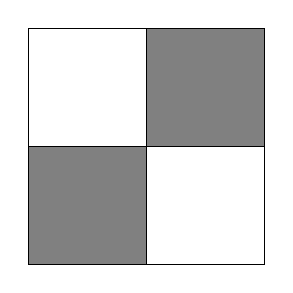
\begin{tikzpicture}	
			\draw [draw=black] (0, 0) rectangle (3, 3);
			\filldraw [draw=black,fill=gray] (0, 0) rectangle (1.5, 1.5);
			\filldraw [draw=black,fill=gray] (1.5, 1.5) rectangle (3, 3);
		\end{tikzpicture}
		\caption{Informative, Lewis-relevant, Roberts-relevant}
	\end{subfigure}\hfill
	\begin{subfigure}[b]{.3\linewidth}
		\centering
		\begin{tikzpicture}	
			\draw [draw=black] (0, 0) rectangle (3, 3);
			\draw [draw=black] (0, 0) rectangle (1.5, 1.5);
			\draw [draw=black] (1.5, 1.5) rectangle (3, 3);
		\end{tikzpicture}
		\caption{Informative, not Lewis-relevant, Roberts-relevant}
	\end{subfigure}\hfill
	\begin{subfigure}[b]{.33\linewidth}
		\centering
		
\begin{tikzpicture}	
			\filldraw [draw=black,fill=gray] (0, 0) rectangle (3, 3);
			\draw [draw=black] (0, 0) rectangle (1.5, 1.5);
			\draw [draw=black] (1.5, 1.5) rectangle (3, 3);
		\end{tikzpicture}
		\caption{Uninformative, Lewis-relevant, not Roberts-relevant.}
	\end{subfigure}
\end{figure}
\begin{figure}[H]\ContinuedFloat
	\begin{subfigure}[b]{.3\linewidth}
		\centering
		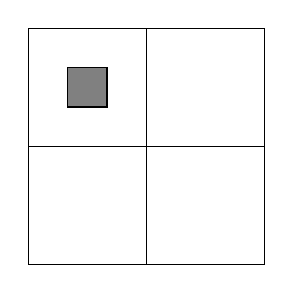
\begin{tikzpicture}	
			\draw [draw=black] (0, 0) rectangle (3, 3);
			\draw [draw=black] (0, 0) rectangle (1.5, 1.5);
			\draw [draw=black] (1.5, 1.5) rectangle (3, 3);
			\filldraw [draw=black,fill=gray] (0.5, 2) rectangle (1,2.5);
		\end{tikzpicture}
		\caption{Informative, not Lewis-relevant, Roberts-relevant}
	\end{subfigure}\hfill
	\begin{subfigure}[b]{.3\linewidth}
		\centering
		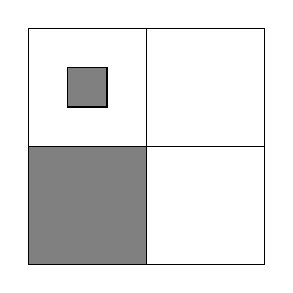
\begin{tikzpicture}	
			\draw [draw=black] (0, 0) rectangle (3, 3);
			\filldraw [draw=black,fill=gray] (0, 0) rectangle (1.5, 1.5);
			\draw [draw=black] (1.5, 1.5) rectangle (3, 3);
			\filldraw [draw=black,fill=gray] (0.5, 2) rectangle (1,2.5);
		\end{tikzpicture}
		\caption{Informative, not Lewis-relevant, Roberts-relevant}
	\end{subfigure}\hfill
	\begin{subfigure}[b]{.33\linewidth}
		\centering
		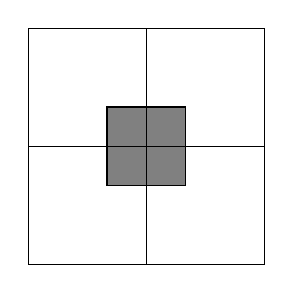
\begin{tikzpicture}	
			\filldraw [draw=black,fill=gray] (1, 1) rectangle (2,2);
			\draw [draw=black] (0, 0) rectangle (3, 3);
			\draw [draw=black] (0, 0) rectangle (1.5, 1.5);
			\draw [draw=black] (1.5, 1.5) rectangle (3, 3);
		\end{tikzpicture}
		\caption{Informative, not Lewis-relevant, not Roberts-relevant}
	\end{subfigure}
\end{figure}


The concept of relevance then directly constrains assertions, given a QuD. If no overt QuD is provided, it is assumed that a reasonable QuD is somehow inferred. This dissertation will focus on how exactly QuDs can be inferred, what additional constraints hold between an assertion and a QuD, and what the consequences are for pragmatic theory.

Specifically, we will claim that instead of being a ``good'' answer to \textit{some} QuD, an out-of-the-blue sentence must be a good answer to a \textit{good} QuD, whose form is determined from the sentence itself. This is pushing the idea that assertions evoke alternatives one step further, in the sense that sentences will be taken to evoke questions (themselves derived from alternatives). These evoked questions will have a structure that consists in a generalization of the partition structure, namely, they will take the form of parse tree of the CS. We will additionally claim the process deriving good questions from good answers, is subject to constraints that go beyond relevance, and cover concepts such as redundancy. These constraints will make way for a ``lifted'' view of pragmatic oddness, under which an assertion is not odd \textit{per se}, but rather, is odd due to its interaction with the QuDs it evokes. Before presenting the core components of our model, we will briefly present two recent accounts of oddness based on similar ideas.














idea that questions and quds are diff
questions may not denote partitions (evidence from embedding, with surprise, surprise whi not p diff from surprise who p)
qud are partitions
=> the two notions are related by a simple mathematical machinery allowng to derive partitions from any set of sets.
null hypothesis: the qud is contextually provided, it's always "out there", or, there is an overt question and the sentence gets matched against it.


inquisiyive semantics says that sentences are more or less questions, they raise issues.
but paradox:sentences and qs are the same kind of thing, but then, sentences get impoverished to be made diff from qs eventually

we explore an alternative (from katzir and singh): we have this idea qs and sentences are linked, but we dont force everything to be in the semantics
 rather, sentences have to obey constraints, that are also influences by the qs the sentnece gives rise to
 

introduce ippolito and stres novelty of account


eahc chapter: say what i will do
do it
say what i have done




\subsection{Background assumptions on question semantics}
I start by reviewing the standard approach to questions. 

Given a CS $S$ and a set of propositions $P$, a partition of $S$ can be generated by grouping together the worlds of $S$ which ``agree'' on all $p \in P$. This is formalized in (\ref{ex:partition-from-propositions}).

\begin{exe}
	\ex {\textit{Partition induced by a set of propositions}. Given a Context Set $S$ and a set of propositions $P$, one can define:
		\begin{itemize}
			\item an equivalence relation $\equiv_P$ s.t. $\forall (w, w') \in S. \ w \equiv_P w' \Leftrightarrow \forall p \in P. \ p(w) = p(w')$
			\item a partition of $S$ induced by $P$, in the form of the set of equivalence classes induced by $\equiv_P$ on $S$, i.e. the set $\lbrace \lbrace w' | w' \in S \wedge w \equiv_P w' \rbrace | w \in S\rbrace$. We call \textsc{Partition}($S$, $P$) the partition of $S$ induced by $P$ in this way. 
	\end{itemize}}\label{ex:partition-from-propositions}
\end{exe}


We can then define the questions evoked by a proposition $p$ as the partitions evoked either by $p$ alone ($P=\lbrace p \rbrace$), or by $p$ and relevant focus alternatives to $p$ ($P=\mathcal{A}_p$) \citep{Rooth1992}. If $p$ is not settled in the CS, the former kind of partition has the form $\lbrace p, \neg p\rbrace$ and amounts to the question of \textit{whether p}. If $\mathcal{A}_p$ contains mutually exclusive, possible propositions covering the CS, then the partition induced by $\mathcal{A}_p$ on the CS is simply $\mathcal{A}_p$, and can be interpreted as a \textit{wh}-question inquiring about $p$'s focus material.

\section{Disjunctions, conditionals, and the QuD}
We start by showing that the felicity of disjunctions and conditionals is sensitive to \textit{overt} QuDs -- but in different ways. We take this as evidence that out-of-the-blue disjunctions and conditionals accommodate different kinds of implicit QuDs.\\

If a context contrasting \textit{Paris} and \textit{France but not Paris} is set as in (\ref{ex:qud-setting}), (\ref{ex:hc-ns-w}) and (\ref{ex:ldhc-ns-w}) improve (cf. \cite{Haslinger2023} for similar effects on disjunctions and conjunctions). This is strange: even if the context and question made \textit{Paris} (but no other French city) a relevant alternative to \textit{France}, \textit{exh} would remain IW in the consequent of (\ref{ex:hc-ns-w}): \textit{if Jo did not grow up in Paris, she grew up in France but not Paris}, is equivalent to \textit{if Jo did not grow up in Paris, she grew up in France}. In other words, \textit{exh} (as constrained by IW) cannot leverage the contextually provided alternatives to make (\ref{ex:hc-ns-w}) escape SR in (\ref{ex:qud-setting}). The same applies to (\ref{ex:ldhc-ns-w}).


\begin{exe}
	\ex{\textit{Context: French accents vary across countries and between Paris the rest of France.}\\
		Al: I'm wondering where Jo learned French.\\
		Lu: I'm not completely sure but... (\ref{ex:hc-ns-w}) \cmark (\ref{ex:ldhc-ns-w}) \cmark}\label{ex:qud-setting}
\end{exe}


This suggests that a purely LF-based view of redundancy such as SR, may be insufficient to capture the interaction between HCs and how their context of utterance packages information. Rather, it seems that the context of (\ref{ex:qud-setting}) makes a specific partition of the CS salient, and that this partition can be used to make otherwise infelicitous assertions accommodate a different question than the one they would evoke out-of-the-blue.

Additionally, conditionals and disjunctions seem to accommodate distinct QuDs. To show this, we use the construction \textit{depending on Q, p} (\cite{Karttunen1977,Kaufmann2016}), where \textit{Q} is a question and \textit{p} a proposition. This construction has been argued to force the partition conveyed by Q to match specific live issues raised by $p$. We understand such ``live issues'' as the maximal true answers of the QuD evoked by $p$. The contrast between (\ref{ex:depending-on-or}) and (\ref{ex:depending-on-if}) then suggests that the \textit{France} and \textit{Belgium} answers can be matched against \textit{Q} in the disjunctive, but not in the conditional case. This in turn means that a disjunction introduces a QuD making both disjuncts maximal true answers, while a conditional does not do the same with its consequent and the negation of its antecedent.

\begin{exe}
	\ex\label{ex:depending-on} Depending on $[$how her accent sounds like$]_{Q}$...
	\begin{xlist}
		\ex {Jo grew up in France \textbf{or} in Belgium. \hfill \p{}$\vee$\q }\label{ex:depending-on-or}
		\ex[??]{\textbf{if} Jo didn't grow up in France she grew up in Belgium. \hfill $\neg$\p{}$\rightarrow$\q} \label{ex:depending-on-if}
		\ex[?] {\textbf{if} Jo didn't grow up in France, she grew up in Belgium \textbf{or} in Québec. \hfill $\neg$\p{}$\rightarrow$(\q$\vee$\r)}\label{ex:depending-on-if-or}
		\ex [??]{\textbf{if} Jo didn't grow up in France \textbf{or} Belgium, she grew up in Québec. \hfill $\neg$(\p$\vee$\q)$\rightarrow$\r}\label{ex:depending-on-or-if}
	\end{xlist}
\end{exe}


The existence of an improvement between (\ref{ex:depending-on-if}) and (\ref{ex:depending-on-if-or}), and the absence of a similar improvement in between (\ref{ex:depending-on-if}) and (\ref{ex:depending-on-or-if}), also implies that the answers targeted by \textit{depending on Q}, when \textit{p} is conditional, are the ones made available by the consequent of \textit{p} (which is appropriately disjunctive in (\ref{ex:depending-on-if-or}), but not (\ref{ex:depending-on-or-if})).




More generally, this predicts ``connectivity effects'' in disjunctions-of-conditionals, in that the antecedents and consequents respectively have to address similar QuDs; and no such effect in conditionals-of-disjunctions, in that disjuncts coming from the antecedent and consequent may be inquisitively unrelated.